Ist es möglich, einen regulären Ausdruck anzugeben, der auf Zeichenketten
der folgenden Form passt?
Eine solche Zeichenkette soll mit einer Anzahl $n$ von Zeichengruppen
\texttt{01} beginnen, gefolgt von genau $n$ Zeichen \texttt{2}.

\thema{Pumping Lemma für reguläre Sprachen}
\thema{regulär}

\begin{loesung}
Dies ist die Sprache 
\[
L = \{ (\texttt{01})^n\texttt{2}^n\,|\, n>0\}.
\]
Sie ist nicht regulär, wie man mit dem Pumping Lemma zeigen kann.
\begin{enumerate}
\item
Dazu nehmen wir an, $L$ sei regulär.
\item
Nach dem Pumping Lemma gibt es eine Zahl $N$, die Pumping Length, derart,
dass jedes Wort $w\in L$ mit Länge $|w|\ge N$ aufgepumpte werden kann.
\item
Wir konstruieren das Wort
\[
w = (\texttt{01})^N\texttt{2}^N
\]
Das Wort $w$ ist offensichtlich in $L$ und $|w|=3N\ge N$.
\item
Nach den Annahmen des Pumping Lemma gibt es eine Aufteilung des
Wortes in drei Teile $w=xyz$, wobei $|xy|\le N$.
Dies zeigt, dass der Teil $y$ vollständig innerhalb des Teils
aus \texttt{01} liegen muss:
\begin{center}
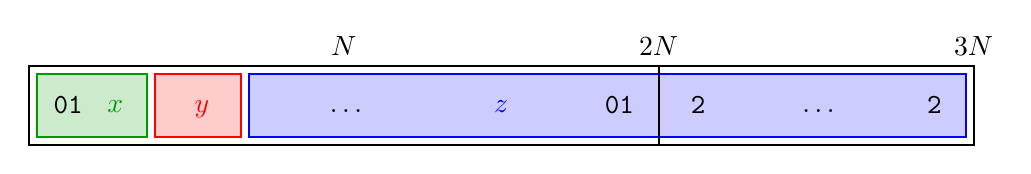
\begin{tikzpicture}[>=latex,thick]
\draw (0,0)--(12,0)--(12,1)--(0,1)--cycle;
\node at (4,1) [above] {$N$};
\node at (8,1) [above] {$2N$};
\node at (12,1) [above] {$3N$};
\definecolor{darkgreen}{rgb}{0,0.6,0}
\fill[color=darkgreen!20] (0.1,0.1) rectangle (1.5,0.9);
\draw[color=darkgreen] (0.1,0.1)--(1.5,0.1)--(1.5,0.9)--(0.1,0.9)--cycle;
\fill[color=red!20] (1.6,0.1) rectangle (2.7,0.9);
\draw[color=red] (1.6,0.1)--(2.7,0.1)--(2.7,0.9)--(1.6,0.9)--cycle;
\fill[color=blue!20] (2.8,0.1) rectangle (11.9,0.9);
\draw[color=blue] (2.8,0.1)--(11.9,0.1)--(11.9,0.9)--(2.8,0.9)--cycle;
\node[color=darkgreen] at (1.1,0.5) {$\mathstrut x$};
\node[color=red] at (2.2,0.5) {$\mathstrut y$};
\node[color=blue] at (6,0.5) {$\mathstrut z$};
\draw (8,0)--(8,1);
\node at (8.5,0.5) {\texttt{2}};
\node at (10,0.5) {$\mathstrut\dots$};
\node at (11.5,0.5) {\texttt{2}};
\node at (0.5,0.5) {\texttt{01}};
\node at (4,0.5) {$\mathstrut\dots$};
\node at (7.5,0.5) {\texttt{01}};
\end{tikzpicture}
\end{center}
\item
Beim Aufpumpen des Teils $y$ ändert die Zahl der Zeichen \texttt{0}
oder \texttt{1}, aber die Anzahl der \texttt{2} ändert nicht.
Ein gepumptes Wort kann also nicht mehr in $L$ sein.
\item
Dieser Widerspruch zeigt, dass die Annahme in Schritt~1 
falsch war, dass also $L$ nicht regulär sein kann.
\qedhere
\end{enumerate}
\end{loesung}

\begin{bewertung}
Für jeden Schritt 1 Punkt.
\end{bewertung}

